\documentclass[tikz,border=12pt]{standalone}
\usepackage[T1]{fontenc}
\usepackage{lmodern}
\usepackage{amsmath}
\usepackage{graphicx}
\usetikzlibrary{arrows.meta,positioning,fit,calc,backgrounds,matrix}

\newcommand{\vlmscoremat}{%
\begin{array}{c@{\;}c}
&
\begin{array}{cccccccc}
\mathbf{k}_1^{\mathrm{img}} \quad &
\mathbf{k}_2^{\mathrm{img}} \quad &
\ldots \quad &
\mathbf{k}_m^{\mathrm{img}} \quad &
\mathbf{k}_1^{\mathrm{txt}} \quad &
\mathbf{k}_2^{\mathrm{txt}} \quad &
\ldots \quad &
\mathbf{k}_n^{\mathrm{txt}}
\end{array}
\\[-1mm]
\begin{array}{c}
\mathbf{q}_1^{\mathrm{img}}\\[2.2mm]
\mathbf{q}_2^{\mathrm{img}}\\[2.2mm]
\vdots\\[2.2mm]
\mathbf{q}_m^{\mathrm{img}}\\[2.2mm]
\mathbf{q}_1^{\mathrm{txt}}\\[2.2mm]
\mathbf{q}_2^{\mathrm{txt}}\\[2.2mm]
\vdots\\[2.2mm]
\mathbf{q}_n^{\mathrm{txt}}
\end{array}
&
{
\renewcommand{\arraystretch}{1.35}
\setlength{\arraycolsep}{6pt}
\begin{bmatrix}
s_{11}^{\mathrm{img,img}} & s_{12}^{\mathrm{img,img}} & \ldots & s_{1m}^{\mathrm{img,img}} &
s_{11}^{\mathrm{img,txt}} & s_{12}^{\mathrm{img,txt}} & \ldots & s_{1n}^{\mathrm{img,txt}}
\\

s_{21}^{\mathrm{img,img}} & s_{22}^{\mathrm{img,img}} & \ldots & s_{2m}^{\mathrm{img,img}} &
s_{21}^{\mathrm{img,txt}} & s_{22}^{\mathrm{img,txt}} & \ldots & s_{2n}^{\mathrm{img,txt}}
\\

\vdots & \vdots & \ddots & \vdots &
\vdots & \vdots & \ddots & \vdots
\\

s_{m1}^{\mathrm{img,img}} & s_{m2}^{\mathrm{img,img}} & \ldots & s_{mm}^{\mathrm{img,img}} &
s_{m1}^{\mathrm{img,txt}} & s_{m2}^{\mathrm{img,txt}} & \ldots & s_{mn}^{\mathrm{img,txt}}
\\

s_{11}^{\mathrm{txt,img}} & s_{12}^{\mathrm{txt,img}} & \ldots & s_{1m}^{\mathrm{txt,img}} &
s_{11}^{\mathrm{txt,txt}} & -\infty & \ldots & -\infty
\\

s_{21}^{\mathrm{txt,img}} & s_{22}^{\mathrm{txt,img}} & \ldots & s_{2m}^{\mathrm{txt,img}} &
s_{21}^{\mathrm{txt,txt}} & s_{22}^{\mathrm{txt,txt}} & \ldots & -\infty
\\

\vdots & \vdots & \ddots & \vdots &
\vdots & \vdots & \ddots & \vdots
\\

s_{n1}^{\mathrm{txt,img}} & s_{n2}^{\mathrm{txt,img}} & \ldots & s_{nm}^{\mathrm{txt,img}} &
s_{n1}^{\mathrm{txt,txt}} & s_{n2}^{\mathrm{txt,txt}} & \ldots & s_{nn}^{\mathrm{txt,txt}}
\end{bmatrix}
}
\end{array}}

\newcommand{\vlmalphamat}{%
{
\renewcommand{\arraystretch}{1.35}
\setlength{\arraycolsep}{6pt}
\begin{bmatrix}
\alpha_{11}^{\mathrm{img,img}} & \ldots & \alpha_{1m}^{\mathrm{img,img}} &
\alpha_{11}^{\mathrm{img,txt}} & \ldots & \alpha_{1n}^{\mathrm{img,txt}}
\\

\alpha_{21}^{\mathrm{img,img}} & \ldots & \alpha_{2m}^{\mathrm{img,img}} &
\alpha_{21}^{\mathrm{img,txt}} & \ldots & \alpha_{2n}^{\mathrm{img,txt}}
\\

\vdots & \ddots & \vdots &
\vdots & \ddots & \vdots
\\

\alpha_{m1}^{\mathrm{img,img}} & \ldots & \alpha_{mm}^{\mathrm{img,img}} &
\alpha_{m1}^{\mathrm{img,txt}} & \ldots & \alpha_{mn}^{\mathrm{img,txt}}
\\

\alpha_{11}^{\mathrm{txt,img}} & \ldots & \alpha_{1m}^{\mathrm{txt,img}} &
\alpha_{11}^{\mathrm{txt,txt}} & \ldots & 0
\\

\alpha_{21}^{\mathrm{txt,img}} & \ldots & \alpha_{2m}^{\mathrm{txt,img}} &
\alpha_{21}^{\mathrm{txt,txt}} & \ldots & 0
\\

\vdots & \ddots & \vdots &
\vdots & \ddots & \vdots
\\

\alpha_{n1}^{\mathrm{txt,img}} & \ldots & \alpha_{nm}^{\mathrm{txt,img}} &
\alpha_{n1}^{\mathrm{txt,txt}} & \ldots & \alpha_{nn}^{\mathrm{txt,txt}}
\end{bmatrix}
}}

\begin{document}
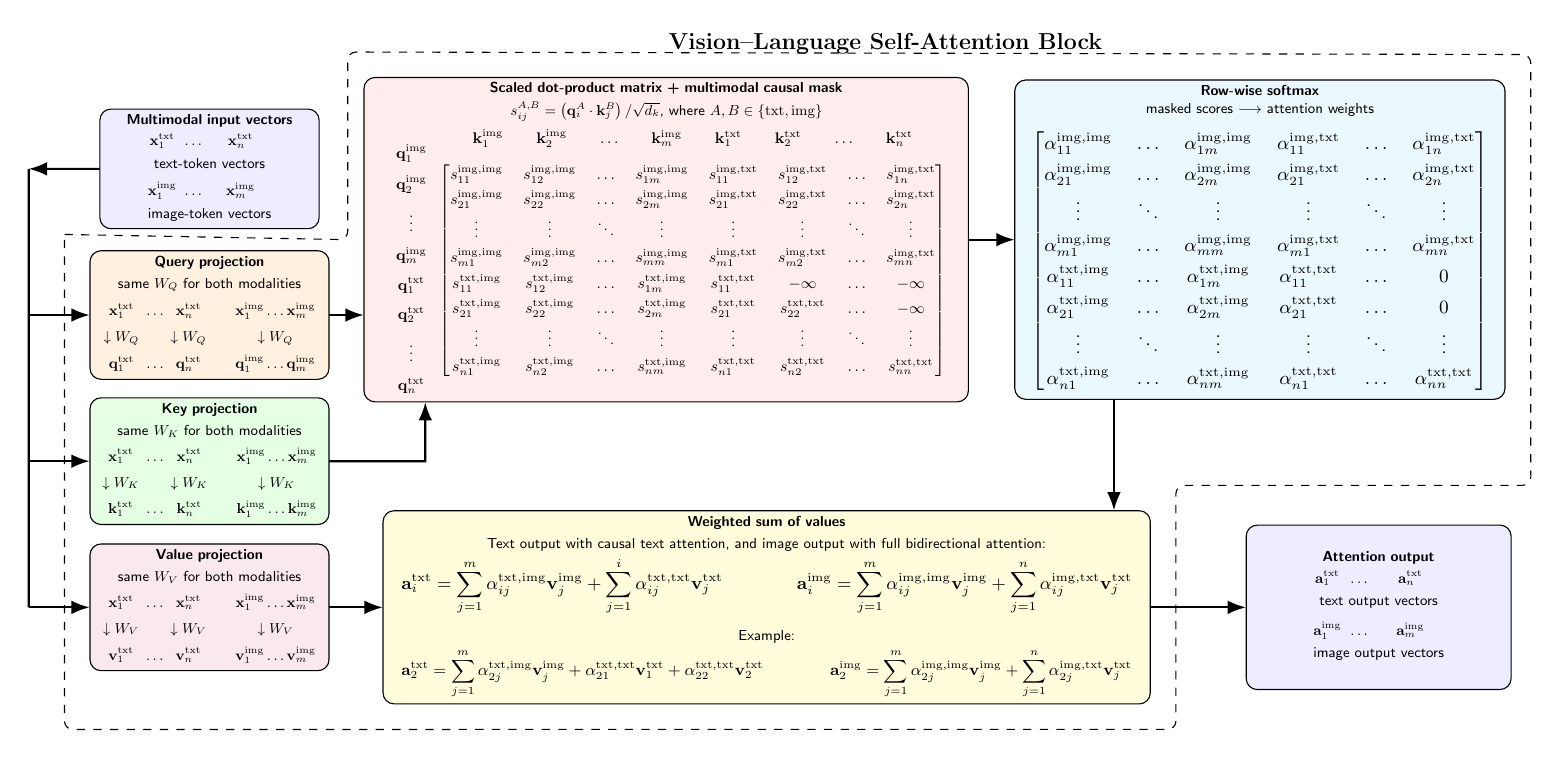
\begin{tikzpicture}[
    scale=0.58,
    every node/.style={transform shape},
    font=\sffamily\small,
    >=Latex,
    arrow/.style={->, thick},
    inputbox/.style={draw, rounded corners=4pt, align=center, fill=blue!7,
        minimum width=4.8cm, text width=4.5cm, minimum height=2.2cm},
    qbox/.style={draw, rounded corners=4pt, align=center, fill=orange!12,
        minimum width=5.0cm, text width=5.0cm, minimum height=2.5cm},
    kbox/.style={draw, rounded corners=4pt, align=center, fill=green!10,
        minimum width=5.0cm, text width=5.0cm, minimum height=2.5cm},
    vbox/.style={draw, rounded corners=4pt, align=center, fill=purple!9,
        minimum width=5.0cm, text width=5.0cm, minimum height=2.5cm},
    scorebox/.style={draw, rounded corners=4pt, align=center, fill=red!7,
        minimum width=12.5cm, text width=13.0cm, minimum height=6.0cm},
    softbox/.style={draw, rounded corners=4pt, align=center, fill=cyan!8,
        minimum width=10.0cm, text width=10.5cm, minimum height=5.3cm},
    outbox/.style={draw, rounded corners=4pt, align=center, fill=yellow!14,
        minimum width=16.8cm, text width=16.5cm, minimum height=4.2cm},
    finalbox/.style={draw, rounded corners=4pt, align=center, fill=blue!7,
        minimum width=5.8cm, text width=5.5cm, minimum height=3.6cm}
]

% Title
\node[font=\bfseries\Large] (title) at (18.0,4.9) {Vision--Language Self-Attention Block};

% Input
\node[inputbox] (input) at (3.2,2.15) {\textbf{Multimodal input vectors}\\[1mm]
{\setlength{\tabcolsep}{2.5pt}
\begin{tabular}{ccc}
$\mathbf{x}_1^{\mathrm{txt}}$ &
$\ldots$ &
$\mathbf{x}_n^{\mathrm{txt}}$
\\[1mm]
\multicolumn{3}{c}{text-token vectors}
\\[2mm]
$\mathbf{x}_1^{\mathrm{img}}$ &
$\ldots$ &
$\mathbf{x}_m^{\mathrm{img}}$
\\[1mm]
\multicolumn{3}{c}{image-token vectors}
\end{tabular}}};

% Q, K, V blocks
\node[qbox] (qproj) at (3.2,-1.05) {\textbf{Query projection}\\[1mm]
same $W_Q$ for both modalities\\[2mm]
{\setlength{\tabcolsep}{2.2pt}
\begin{tabular}{ccccc}
$\mathbf{x}_1^{\mathrm{txt}}$ &
$\ldots$ &
$\mathbf{x}_n^{\mathrm{txt}}$ &
$\quad$ &
$\mathbf{x}_1^{\mathrm{img}} \ldots \mathbf{x}_m^{\mathrm{img}}$
\\[1.8mm]
$\downarrow W_Q$ &
&
$\downarrow W_Q$ &
&
$\downarrow W_Q$
\\[1.8mm]
$\mathbf{q}_1^{\mathrm{txt}}$ &
$\ldots$ &
$\mathbf{q}_n^{\mathrm{txt}}$ &
$\quad$ &
$\mathbf{q}_1^{\mathrm{img}} \ldots \mathbf{q}_m^{\mathrm{img}}$
\end{tabular}}};

\node[kbox] (kproj) at (3.2,-4.25) {\textbf{Key projection}\\[1mm]
same $W_K$ for both modalities\\[2mm]
{\setlength{\tabcolsep}{2.2pt}
\begin{tabular}{ccccc}
$\mathbf{x}_1^{\mathrm{txt}}$ &
$\ldots$ &
$\mathbf{x}_n^{\mathrm{txt}}$ &
$\quad$ &
$\mathbf{x}_1^{\mathrm{img}} \ldots \mathbf{x}_m^{\mathrm{img}}$
\\[1.8mm]
$\downarrow W_K$ &
&
$\downarrow W_K$ &
&
$\downarrow W_K$
\\[1.8mm]
$\mathbf{k}_1^{\mathrm{txt}}$ &
$\ldots$ &
$\mathbf{k}_n^{\mathrm{txt}}$ &
$\quad$ &
$\mathbf{k}_1^{\mathrm{img}} \ldots \mathbf{k}_m^{\mathrm{img}}$
\end{tabular}}};

\node[vbox] (vproj) at (3.2,-7.45) {\textbf{Value projection}\\[1mm]
same $W_V$ for both modalities\\[2mm]
{\setlength{\tabcolsep}{2.2pt}
\begin{tabular}{ccccc}
$\mathbf{x}_1^{\mathrm{txt}}$ &
$\ldots$ &
$\mathbf{x}_n^{\mathrm{txt}}$ &
$\quad$ &
$\mathbf{x}_1^{\mathrm{img}} \ldots \mathbf{x}_m^{\mathrm{img}}$
\\[1.8mm]
$\downarrow W_V$ &
&
$\downarrow W_V$ &
&
$\downarrow W_V$
\\[1.8mm]
$\mathbf{v}_1^{\mathrm{txt}}$ &
$\ldots$ &
$\mathbf{v}_n^{\mathrm{txt}}$ &
$\quad$ &
$\mathbf{v}_1^{\mathrm{img}} \ldots \mathbf{v}_m^{\mathrm{img}}$
\end{tabular}}};

% Matrix blocks
\node[scorebox] (scores) at (13.2,0.6) {\textbf{Scaled dot-product matrix + multimodal causal mask}\\[1mm]
\begin{tabular}{c}
$s_{ij}^{A,B}
=
\left(\mathbf{q}_i^{A}\cdot \mathbf{k}_j^{B}\right)/
\sqrt{d_k}
$,
where $A,B\in\{\mathrm{txt},\mathrm{img}\}$\\[2mm]
\resizebox{12.6cm}{!}{$\vlmscoremat$}
\end{tabular}};

\node[softbox] (softmax) at (26.2,0.6) {\textbf{Row-wise softmax}\\[1mm]
\begin{tabular}{c}
masked scores $\longrightarrow$ attention weights\\[2mm]
\resizebox{10.0cm}{!}{$\vlmalphamat$}
\end{tabular}};

% Weighted values block
\node[outbox] (weighted) at (15.4,-7.45) {\textbf{Weighted sum of values}\\[1mm]
Text output with causal text attention, and image output with full bidirectional attention:\\[1mm]
\resizebox{16.0cm}{!}{$\displaystyle
\mathbf{a}_i^{\mathrm{txt}}
=
\sum_{j=1}^{m}
\alpha_{ij}^{\mathrm{txt,img}}\mathbf{v}_j^{\mathrm{img}}
+
\sum_{j=1}^{i}
\alpha_{ij}^{\mathrm{txt,txt}}\mathbf{v}_j^{\mathrm{txt}}
\qquad\qquad
\mathbf{a}_i^{\mathrm{img}}
=
\sum_{j=1}^{m}
\alpha_{ij}^{\mathrm{img,img}}\mathbf{v}_j^{\mathrm{img}}
+
\sum_{j=1}^{n}
\alpha_{ij}^{\mathrm{img,txt}}\mathbf{v}_j^{\mathrm{txt}}
$}\\[3mm]
Example:\\[1mm]
\resizebox{16.0cm}{!}{$\displaystyle
\mathbf{a}_2^{\mathrm{txt}}
=
\sum_{j=1}^{m}
\alpha_{2j}^{\mathrm{txt,img}}\mathbf{v}_j^{\mathrm{img}}
+
\alpha_{21}^{\mathrm{txt,txt}}\mathbf{v}_1^{\mathrm{txt}}
+
\alpha_{22}^{\mathrm{txt,txt}}\mathbf{v}_2^{\mathrm{txt}}
\qquad\qquad
\mathbf{a}_2^{\mathrm{img}}
=
\sum_{j=1}^{m}
\alpha_{2j}^{\mathrm{img,img}}\mathbf{v}_j^{\mathrm{img}}
+
\sum_{j=1}^{n}
\alpha_{2j}^{\mathrm{img,txt}}\mathbf{v}_j^{\mathrm{txt}}
$}
};

% Output
\node[finalbox] (output) at (28.8,-7.45) {\textbf{Attention output}\\[1mm]
{\setlength{\tabcolsep}{2.8pt}
\begin{tabular}{ccc}
$\mathbf{a}_1^{\mathrm{txt}}$ &
$\ldots$ &
$\mathbf{a}_n^{\mathrm{txt}}$
\\[1mm]
\multicolumn{3}{c}{text output vectors}
\\[2.5mm]
$\mathbf{a}_1^{\mathrm{img}}$ &
$\ldots$ &
$\mathbf{a}_m^{\mathrm{img}}$
\\[1mm]
\multicolumn{3}{c}{image output vectors}
\end{tabular}}};

% Input arrows
\coordinate (inputtrunktop) at ($(input.west)+(-1.55,0)$);
\coordinate (inputtrunkbottom) at (inputtrunktop |- vproj.west);

\draw[arrow] (input.west) -- (inputtrunktop);
\draw[thick] (inputtrunktop) -- (inputtrunkbottom);

\draw[arrow] (inputtrunktop |- qproj.west) -- (qproj.west);
\draw[arrow] (inputtrunktop |- kproj.west) -- (kproj.west);
\draw[arrow] (inputtrunktop |- vproj.west) -- (vproj.west);

% Query into the score block
\draw[arrow] (qproj.east) -- (scores.west |- qproj.east);

% Key into the score block
\coordinate (keybend) at ($(kproj.east)+(2.1,0)$);
\draw[arrow] (kproj.east) -- (keybend) -- (keybend |- scores.south);

% Scores to softmax
\draw[arrow] (scores.east) -- (softmax.west);

% Softmax to weighted sum
\coordinate (softToWeighted) at ($(softmax.south)+(-3.2,0)$);
\draw[arrow] (softToWeighted) -- (softToWeighted |- weighted.north);

% Value projection to weighted sum
\draw[arrow] (vproj.east) -- (weighted.west);

% Weighted sum to output
\draw[arrow] (weighted.east) -- (output.west);

% Dashed background outline:
% Orthogonal polygon with a fully horizontal bottom edge.
\begin{pgfonlayer}{background}
\coordinate (outlineA) at ($(qproj.north west)+(-0.55,0.35)$);
\coordinate (outlineB) at ($(scores.west)+(-0.35,0)$ |- outlineA);
\coordinate (outlineC) at ($(scores.north west)+(-0.35,0.55)$);
\coordinate (outlineD) at ($(softmax.north east)+(0.55,0.55)$);
\coordinate (outlineE) at ($(softmax.south east)+(0.55,-0.55)$);
\coordinate (outlineG) at ($(weighted.north east)+(0.55,0.55)$);
\coordinate (outlineF) at (outlineE |- outlineG);
\coordinate (outlineH) at ($(weighted.south east)+(0.55,-0.55)$);
\coordinate (outlineJ) at (outlineA |- outlineH);

\draw[dashed, rounded corners=3pt]
    (outlineA)
    --
    (outlineB)
    --
    (outlineC)
    --
    (outlineD)
    --
    (outlineE)
    --
    (outlineF)
    --
    (outlineG)
    --
    (outlineH)
    --
    (outlineJ)
    --
    (outlineA);
\end{pgfonlayer}

\end{tikzpicture}
\end{document}